\chapter{Experimental Verification}

\section{Sample Preperation}
Magnetite Nanoparticles coated with Oleic Acid dispersed in Toluene were bought from NN-Labs, Inhibited Methylmethacrylate (MMA) and Etyhlhexylmethacrylate (EHMA)  (Sigma Aldrich) were filtered using a prefilled column to remove the Inhibitor.  2,2 azo-bis-isobutyrylnitrile (AIBN) (Sigma Aldrich) was used as initiator as received. Polystyrene (Sigma Aldrich, MW XXX) was used as received. As solvents, Methanol, Toluene and Chloroform were used.
\subsection{Nanoparticles in Polystyrene Matrix}
The nanoparticles were precipitated with MeOH, centrifuged and redispersed in Chloroform at a concentration of 25\,mg/ml, whereas the weight of nanoparticles includes the weight of the oleic acid capping. Polystyrene was dissolved in Chloroform at a concentration of 250\,mg/ml and different volumes of the nanoparticles solution were added (to account for the different iron contents) to 5\,ml of the Polystyrene solution (see \fref{tab:samplePS}). After ensuring dispersion by strong sonication, fractions of XXX\,ul the solution were dropped onto glass slides and dried. After drying, the films were carefully removed from the glass slides.
As an iron containing control sample, 60mg FeCl3 and XXX Polystyrene were dissolved in 6ml acetone, sonicated and  fractions of XXX were dropped onto slowly spinning glass slides (XXX rpm for XX 5\,min) and carefully removed after drying.
\begin{table}
	\centering
	\caption{Nanoparticles in Polystyrene recipes}
	\label{tab:samplePS}
	\begin{tabular}{llll}
		\hline
	NP size&   Volume NP in CF &  Iron Concentration &Volume PS in CF    \\
		\hline
	  5\,nm&700 ul & & 5\,ml  \\  
	   10\,nm&  500 ul& &5\,ml  \\    
	   20\,nm &  425 ul& &5\,ml  \\  
	   	Control   &  & &5\,ml  \\  
		\hline
	\end{tabular}
\end{table}

\subsection{Nanoparticles in Poly(MMA/EHMA)  Matrix}
As a second nanoparticle in polymer sample, a AIBN initiated Poly(MMA/EHMA) polymerisation with magnetite nanoparticles was performed. 
The nanoparticle solution was concentrated to XXX in Tolune by precipitation and redispersion. To account for the different iron concentration, to different amounts of the nanoparticle solution and toluene 800\,ul of EHMA was added each (see \fref{tab:sampleCP}). After strong sonication to ensure dispersion, 3.2\,ml of MMA were added and the solution was bubbled with N$_2$ for 5\,min. To start the polymerisation, 20\,mg of AIBN were added and the solution was bubbled with N$_2$  for 10\,min before moving heating it up to XXX using a water bath under weak sonication. The mixture was keept at XXX for XXX.
The vials were uncapped and the polymer dried for 12h at XXX. The polymer was removed from the vials and cut into slices using a slow spinning diamond saw.
As a control sample, the polymerisation was performed without any nanoparticles. 

\begin{table}
	\centering
	\caption{Nanoparticles in PMMA/EHMA recipes}
	\label{tab:sampleCP}
	\begin{tabular}{llllll}
		\hline
		NP size &NP in Toluene&Toluene & EHMA & MMA & AIBN \\
		\hline
		5\,nm& & &800\,ul&  3.2\,ml&   20\,mg    \\
		10\,nm& & &800\,ul&  3.2\,ml&   20\,mg    \\
		10\,nm& & &0\,ul&  4\,ml&   20\,mg    \\
		20\,nm& & &800\,ul&  3.2\,ml&   20\,mg    \\
			Control& & 1\,ml&800\,ul&  3.2\,ml&   20\,mg    \\
		\hline
	\end{tabular}
\end{table}

\subsection{Sample Characterisation}
\subsection{GaAs crystal films}

\section{Setup}
\begin{figure}
	\centering
	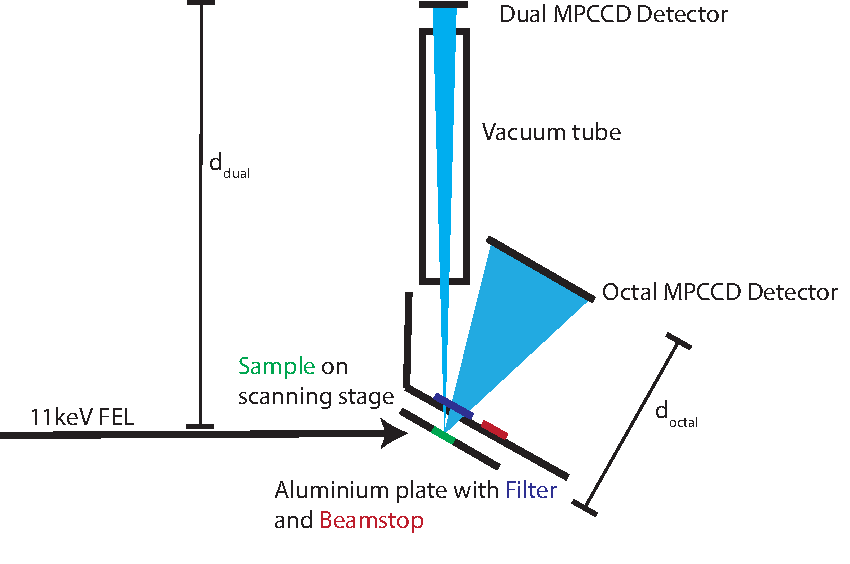
\includegraphics[width=0.8\linewidth]{images/setup.pdf}
	\caption{Schematic of the experimental setup at SACLA}
\end{figure}
\subsection{Imaging the Focus}
\subsection{Imaging Nanoparticles}
\subsection{Imaging Crystals}

\section{Results}
\subsection{Imaging the Focus}
\subsubsection{Filtering}

\subsection{Imaging Nanoparticles}
\subsubsection{Filtering}
\subsection{Imaging Crystals}
\subsubsection{Crystal orientation}


